\chapter{Manuales}\label{chap:manual}

\section{Manual de usuario}\label{sec:manual_usuario}


\newpage{}
\section{Manual de despliegue}\label{sec:manual_despliegue}
El sistema se ha diseñado para llevar la menor cantidad de pasos posible en su
instalación. Debido a la colección de tecnologías utilizadas, (Terraform,
Docker y ECS), el despliegue de la infraestructura base requiere la ejecución de
tan solo dos comandos\footnote{Asumiendo que se cumplen los requisitos previos.}.

El sistema de despliegue está pensado para ser ejecutado en un sistema operativo
UNIX, como Linux o macOS. Para su ejecución en Windows, se recomienda el uso
de WSL2\footnote{\url{https://learn.microsoft.com/es-es/windows/wsl/about}}.


\subsection{Requisitos previos}
Previa al despliegue del sistema, se deben cumplir una serie de requisitos
mínimos:


\paragraph{Terraform}
El proceso de instalación de Terraform es sencillo y se puede realizar siguiendo
las instrucciones de la aplicación en su página web oficial\footnote{\url{
	https://developer.hashicorp.com/terraform/install
}} para el sistema operativo que se desee. Una vez descargado e instalado,
se puede comprobar que la instalación ha sido correcta ejecutando el comando
\texttt{terraform -v} en la terminal de comandos del sistema.

\begin{figure}[H]
	\centering
	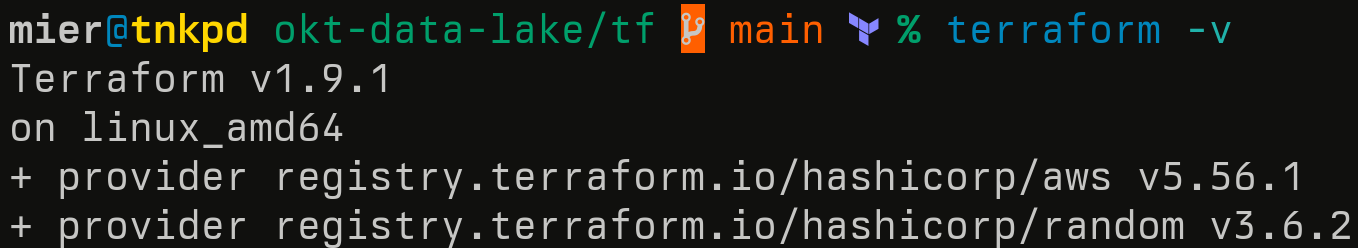
\includegraphics[width=\textwidth]{manual/terraform_v.png}
	\caption{Comprobación de la versión de Terraform}
	\label{fig:terraform_version}
\end{figure}


\newpage{}
\paragraph{Usuario de AWS}
Para poder ejecutar los comandos de Terraform con los permisos necesarios, se
debe disponer de un usuario de AWS con los permisos necesarios para la creación
de los recursos. Se recomienda la creación de un usuario específico para el
despliegue del sistema, con los roles y políticas estrictamente necesarias, para
evitar posibles problemas de seguridad.

Para permitir la interacción con la consola de AWS, se debe instalar la
herramienta de terminal de Amazon\footnote{\url{https://aws.amazon.com/es/cli/}}.

Una vez creado o seleccionado el usuario deseado, se debe inciar sesión en la
consola a través del comando \texttt{aws configure} y seguir las instrucciones
para introducir las credenciales de acceso al sistema.

\begin{figure}[H]
	\centering
	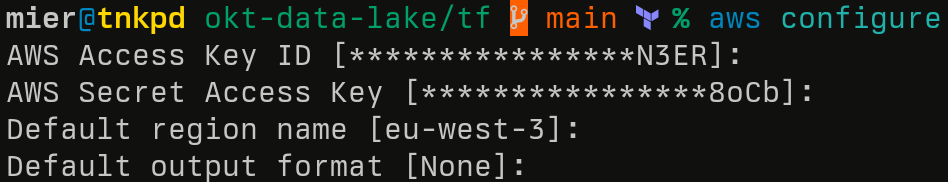
\includegraphics[width=\textwidth]{manual/aws_configure.png}
	\caption{Configuración de credenciales en AWS CLI}
	\label{fig:aws_configure}
\end{figure}

AWS pone a disposición de los usuarios una guía de inicio rápido\footnote{\url{
	https://docs.aws.amazon.com/es_es/cli/latest/userguide/cli-configure-quickstart.html
}} para la configuración de las credenciales.

\begin{figure}[H]
	\centering
	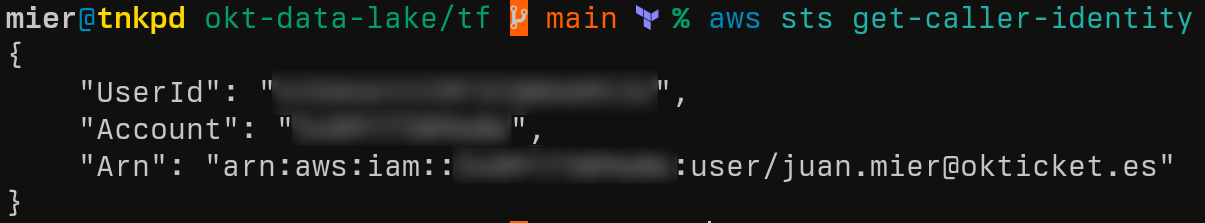
\includegraphics[width=\textwidth]{manual/aws_user.png}
	\caption{Demostración de credenciales en AWS CLI}
	\label{fig:aws_user}
\end{figure}


\newpage{}
\paragraph{Certificados}
Para que funcionen correctamente los servicios de la aplicación mediante HTTPS,
se deben disponer de certificados separados tanto para el dominio y los
recursos de AWS como para los servicios de la aplicación.

Los certificados de AWS se generan automáticamente con el script mediante el
servicio de ACM, mientras que los certificados de la aplicación se deben
generar previamente y almacenar en la carpeta \texttt{certs} del proyecto.

Para la generación de los certificados de la aplicación, se reutiliza los
scripts de preparación de los contenedores del \fullref{sec:impl_local}.
Para la generación de los certificados de la aplicación, se debe ejecutar
el script \texttt{certs.sh} que se encuentra en \fullref{anexo:certificados} o
bien se pueden reutilizar los certificados generados en el despliegue local.

Estos certificados deben ser almacenados en la carpeta \texttt{certs} junto a
los scripts de despliegue de Terraform, y deben tener visibilidad suficiente
para que Terraform pueda acceder a ellos.


\subsection{Despliegue}
Una vez cumplidos los requisitos previos, se puede proceder al despliegue de
la infraestructura base. Para ello, se deben ejecutar los siguientes comandos
desde la carpeta de scripts de Terraform a través de la terminal del sistema:

\begin{lstlisting}
terraform init  # Necesario solo la primera ejecucion
terraform apply
\end{lstlisting}

\begin{figure}[H]
	\centering
	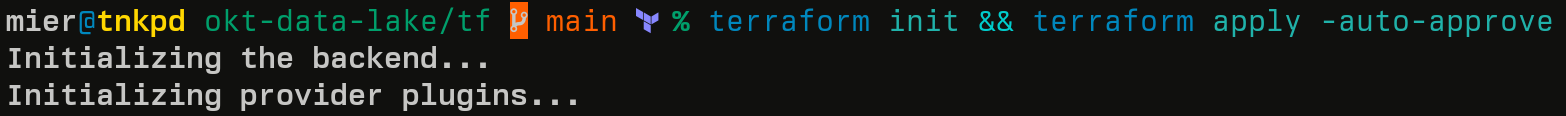
\includegraphics[width=\textwidth]{manual/terraform_apply.png}
	\caption{Despliegue de la infraestructura base}
	\label{fig:terraform_apply}
\end{figure}

El comando \texttt{terraform init} se encarga de inicializar el directorio de
trabajo de Terraform, descargando los módulos necesarios para el despliegue.
El comando \texttt{terraform apply} se encarga de desplegar la infraestructura
base en la cuenta de AWS asociada a las credenciales configuradas en la
herramienta de AWS CLI.

Una vez ejecutado el comando, se mostrará un resumen de los recursos que se
van a crear y se pedirá confirmación para proceder con el despliegue. Para
confirmar, se debe introducir \texttt{yes} y pulsar la tecla \texttt{Enter}.
Una vez confirmado, Terraform procederá a la creación de los recursos de manera
automatizada.

Una vez concluido el despliegue, se mostrará un mensaje de éxito y se devolverán
algunos datos relevantes sobre los recursos creados, como direcciones URL,
identificadores o contraseñas de acceso creadas de manera aleatoria.

\begin{figure}[H]
	\centering
	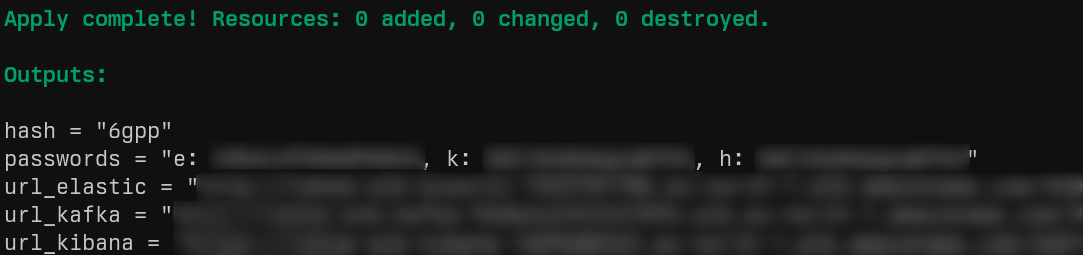
\includegraphics[width=\textwidth]{manual/terraform_output.png}
	\caption{Despliegue exitoso de la infraestructura base}
	\label{fig:terraform_output}
\end{figure}
